\documentclass[11pt]{article}
\usepackage[utf8]{inputenc}
\usepackage{graphicx}
\usepackage{url}
\usepackage{amsmath}
\usepackage{float}


\title{
	{Computer Vision 1 - Assignment 2 \\
	Linear Filters: Gaussians and Derivatives}
}
\author{
Selene Baez Santamaria (10985417) - Andrea Jemmett (11162929)}
\date{\today}

\begin{document}

\maketitle

\section{Harris Corner Detector}
% Question: "Demo function"
To implement the Harris Corner Detector we decided to use the function we implemented on previous assignments. This way we can exploit the benefits of kernel separability and improve performance. Thus, we create horizontal and vertical Gaussian kernels, and apply a Gaussian first order derivative kernel to the image, read in a gray scale format. The image gradients are shown in Figure \ref{fig:partialDerivatives_pingpong} and \ref{fig:partialDerivatives_person}.

\begin{figure}[H] \centering
	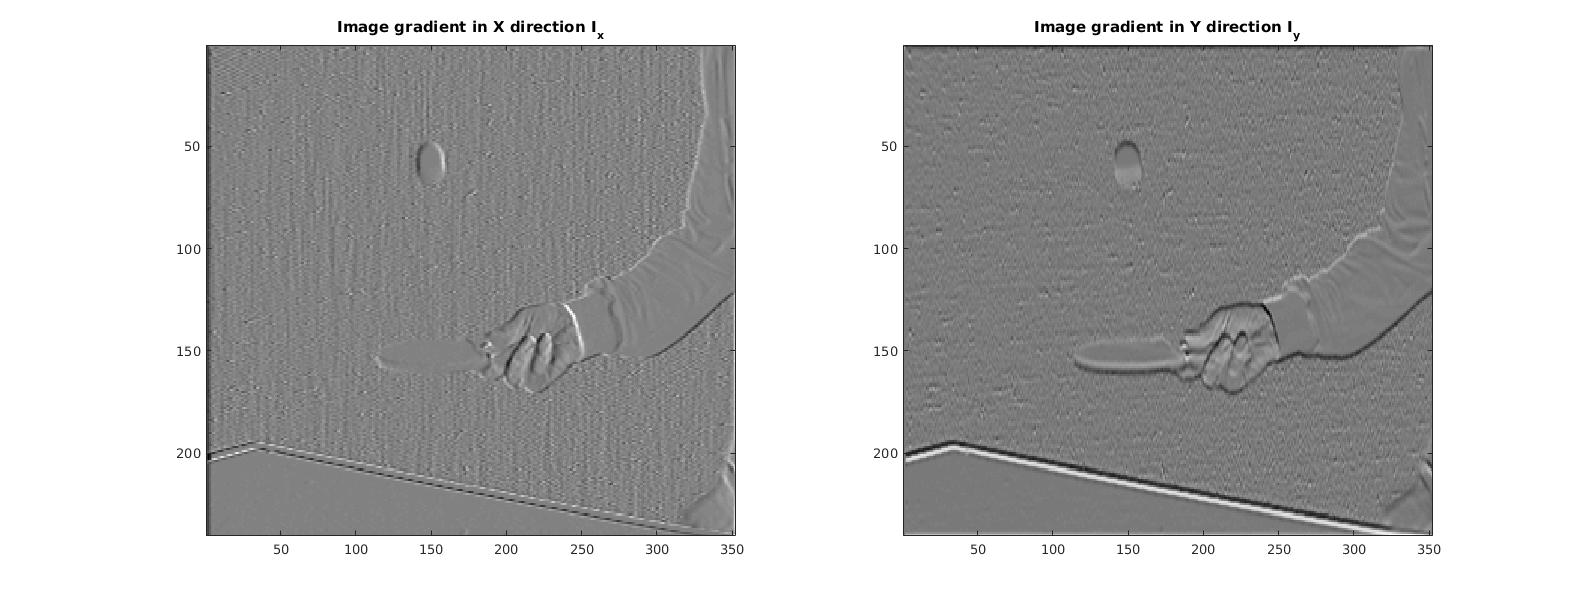
\includegraphics[width=1\textwidth]{imgs/derivatives_pingpong.jpg}
	\caption{Image gradients for first Ping Pong image}
	\label{fig:partialDerivatives_pingpong}
\end{figure}

\begin{figure}[H] \centering
	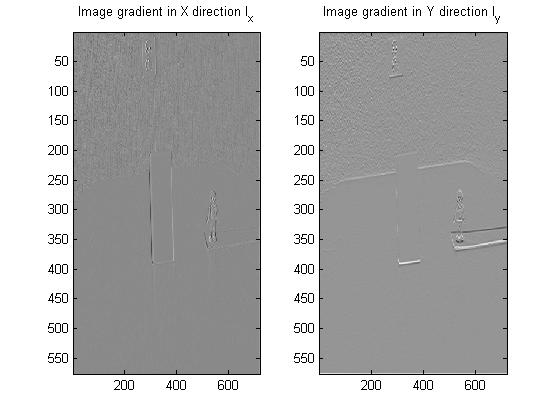
\includegraphics[width=1\textwidth]{imgs/derivatives_person.jpg}
	\caption{Image gradients for first Toy Person image}
	\label{fig:partialDerivatives_person}
\end{figure}

Then, we create the $Q$ matrix, first by squaring raising the gradients (i.e. ($I_x)^2$ and ($I_y)^2$) and multiplying them with each other (i.e. $I_x * I_y$), and then by convolving the resulting with a Gaussian kernel. With these components qe are able to compute $H$ using Equation $12$ shown in the assignment instructions. A visualization for the scaled surfaces are shown in Figure and  .

\begin{figure}[H] \centering
	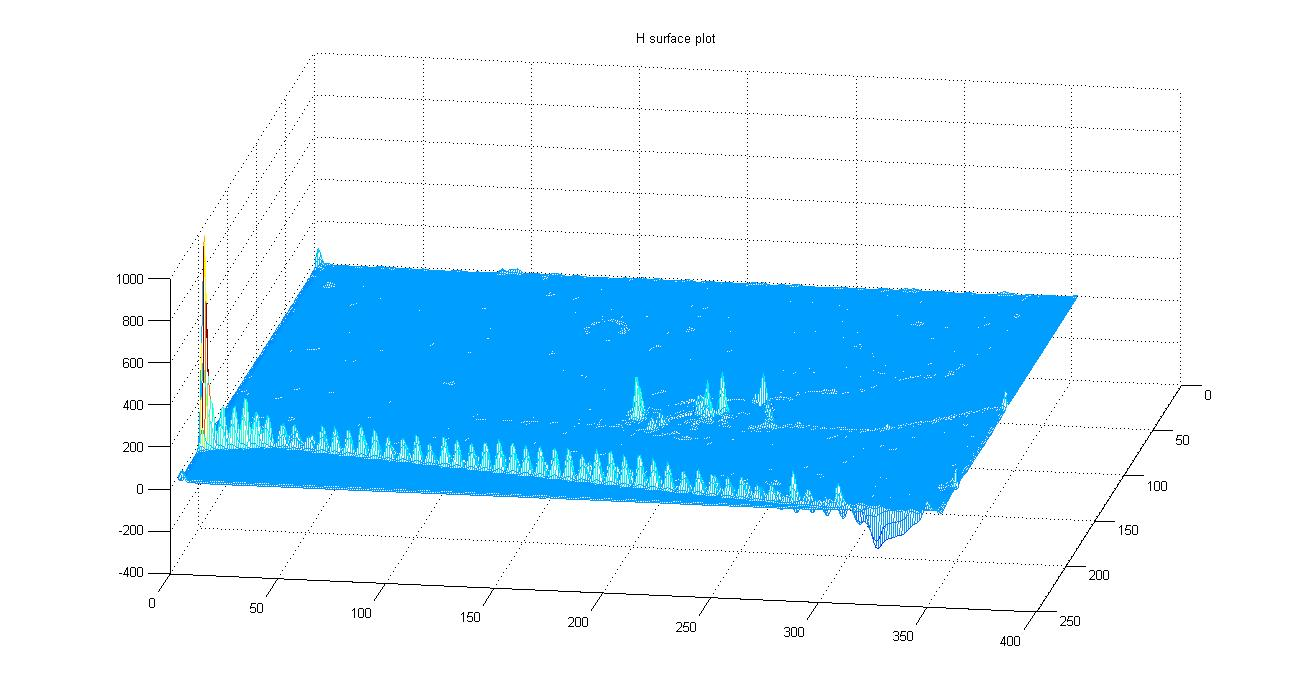
\includegraphics[width=1\textwidth]{imgs/surface_pingpong.jpg}
	\caption{$H$ surface for first Ping Pong image. Local maxima are observed along the ping pong table, and the hand.}
	\label{fig:surface_pingpong}
\end{figure}

\begin{figure}[H] \centering
	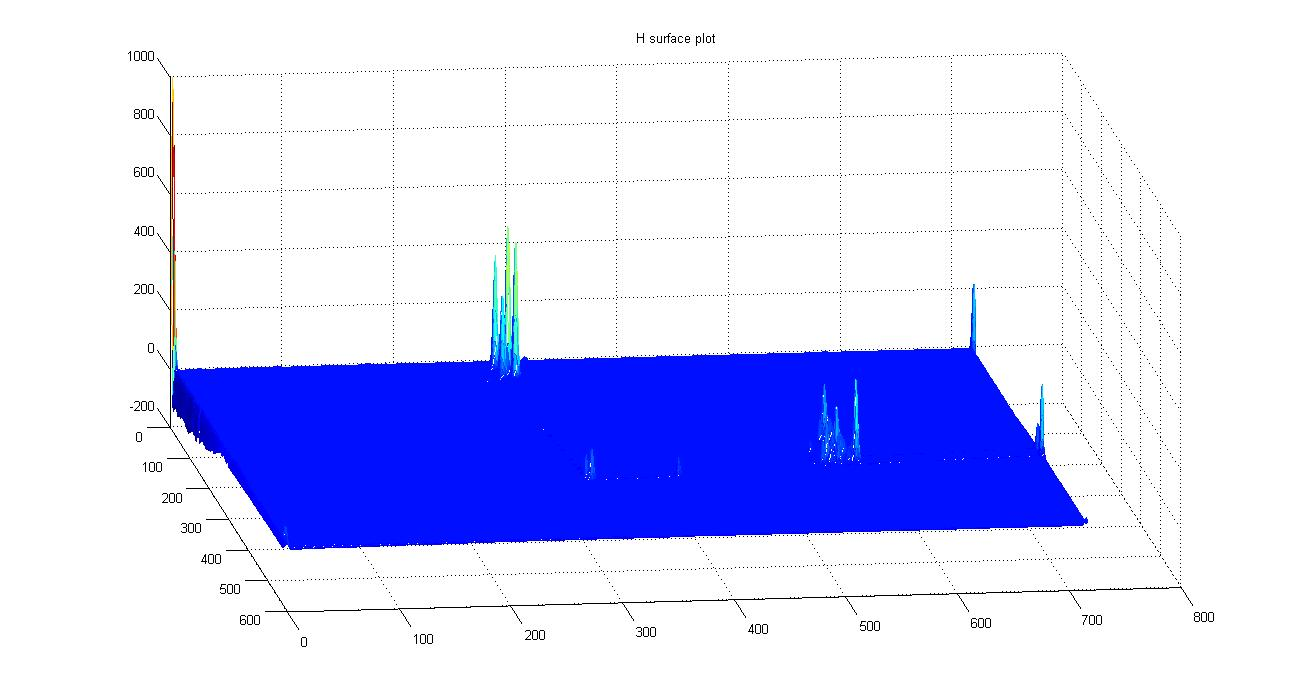
\includegraphics[width=1\textwidth]{imgs/surface_person.jpg}
	\caption{$H$ surface for first Toy Person image. Local maxima are observed on the power outlet and on the toy person.}
	\label{fig:surface_person}
\end{figure}

Finally, to choose the corner points we consider two conditions: 
\begin{enumerate}
	\item A corner point must be a local maximum. To check for this we need to compare its value with all its neighbors' within a given window parameter.
	\item A corner point must have a higher $H$ value than a given threshold. 
\end{enumerate}


To validate our detector we compare it with the Matlab corner function




After tuning, the chosen values for the final detector are: 
\begin{itemize}
	\item $kernel  length = 11$
	\item $\sigma = 1$
	\item $window  size = 3$
	\item $threshold = 7$ 
\end{itemize}

As stated in the previous assignment, a $kernel length$ of 11 and $\sigma$ of 1 seem to work well as parameters for convolving the Gaussian first order derivative kernel to find edges. 

During tuning we discovered the effect of the parameters over the performance of the detector. We noticed that smaller $\sigma$ had an effect of detecting more corner points on the background. A higher threshold reduces the number of corner points and 

a larger window size makes the corner points more sparse, and prevents the corner points to be clustered. 

\section{Lucas-Kanade Algorithm for Optical Flow}



\section{Tracking}

\end{document}